\documentclass[../main/main.tex]{subfiles}
\begin{document}
%\dominitoc
%\faketableofcontents
\setcounter{chapter}{2}
\chapter{Un spectrographe 3D: La Spectral Energy Distribution machine}\label{ch:sedm}

\minitoc
\vspace{2cm}
Dans le chapitre précédent, nous avons présenté la collaboration Zwicky
Transient Facility et nous nous sommes focalisés sur la caméra
principale de $47\text{deg}^{2}$ montée sur le P48 au Mont
Palomar. Cette caméra permet à ZTF de détecter $10^{5}$ évènements
transitoires ou variables, en scannant l'entièreté du ciel Nord visible
chaque nuit,  à la vitesse
vertigineuse de $3760\text{deg}^{2}$/heure. Parmi ces évènements,
$\mathcal{O}(10)$ correspondent à de nouveux évènements transitoires non
répertoriés: Les Supernovae. Comme expliqué dans le
Chapitre~\ref{sec:snia}, seules les Supernovae de type Ia sont
d'intérêts dans la cosmologie, de part leur propriété de chandelle
standardisable. Il faut donc les classifier. Pour cela on utilise leur
spectre, dont les raies d'absorption/émission sont caractéristiques d'un
type à l'autre de SN. Ainsi, ZTF possède également un spectrographe 3D
monté sur le télescope P60 au Mont Palomar
(Figure~\ref{fig:palomar_obs}) spécialement conçu à cet effet. Nous
présentons dans ce chapitre ce spectrographe, la Spectral Energy
Distribution machine (SEDm).
\newpage

\section{Présentation de l'instrument}
\label{sec:ifs}

\subsection{Principe d'un IFS}
Le spectrographe 3D SEDm est ce qu'on appelle un IFS pour Integral Field
Spectrograph. Sans surprise, c'est un instrument qui permet de
recueillir le spectre du ciel sur un champ de vue bidimensionnel.
Ainsi et indépendamment de la méthode utilisée, le produit final avec
cet instrument correspond à
un cube de données ayant 2 dimensions spatiales (($x$, $y$) ou (RA,
Dec) ) et une dimension spectrale (longueur d'onde $\lambda$ ou une
vitesse). Dans tout le manuscrit, cette notion de 3D/cube 3D fera
systématiquement référence aux dimensions ''$x$, $y$, $\lambda$''.

Un IFS est composé de 2 parties: le spectrographe qui va disperser la
lumière incidente, et l'IFU (Integrated Field Unit). Le rôle de l'IFU
est de diviser le plan spatial 2D du champ de vue en un réseau continu
et concentré de lumière. Ce réseau est ensuite donné en entrée au
spectrographe qui va se charger de le disperser sur le détecteur.

Il existe 3 types principaux d'IFU, schématisés dans la Figure~\ref{fig:ifsgeneral}.
\begin{itemize}[label=$\bullet$]
\itemsep0em 
\item \textbf{Le réseau de micro-lentilles} conceptualisé par
  \citet{BaconIFUlens} (qui s'apparente aux yeux composites
  de certains insectes): C'est le système utilisé par la SEDm, mais
  également par l'IFS SAURON \citep{SAURONifs} dans le projet ATLAS3D
  \citep{ATLAS3D} ou encore SNIFS \citep{SNIFS2004}. Dans ce système,
  l'image bi-dimensionnelle est fractionnée par un réseau de
  micro-lentilles (le MLA, microlens array). Chaque élément est ensuite
  concentré et dispersé par le spetrographe (voir
  Figure~\ref{fig:ifsgeneral}). Pour éviter au maximum le chevauchement des
  spectres sur le détecteur, le réseau de lentille est légèrement
  incliné. Le désavantage principal de cette technique est le court
  intervalle de longueur d'onde dispersable sans induire de chevauchement.
  
\item \textbf{Le paquet de fibre} comme
  avec l'IFS du relevé MaNGA d'SDSS \citep{SDSSIFS} qui peut
  être utilisé en combinaison \citep{BardenIFUfiber} ou non
  \citep{allingtonIFUlensfiber} de réseau de micro-lentilles.
  Ici la lumière n'est pas concentrée par des lentilles mais acheminée
  par un paquet de fibres optiques ``à la chaîne'' jusqu'à la fente du spectrographe. Le
  premier avantage est bien évidemment la flexibilité des fibres. Mais
  en contrepartie l'échantillon du ciel disperé devient non contigu, à
  cause de la forme circulaire des fibres. Il est possible de pallier à
  cet effet un ajoutant un réseau de micro-lentilles (lui contigu) entre
  le plan focal et le paquet de fibres.  
  
\item \textbf{Le ``trancheur d'image''} qui est la méthode la plus
  ancienne (\citet{BowenIFUslicer}, \citet{ContentIFUslicer}) utilisée
  par exemple avec le NIFS
  (near-infrared integral field spectrograph, \citet{GeminiNIFS}). Cette
  méthode utilise un mirroir segmenté en fines sections
  horizontales. Chacune de ces sections va diriger la lumière incidente
  dans des directions légèrement différentes jusqu'à un second miroir
  segmenté. Ce dernier va réarranger les tranches incidentes non pas
  l'une au dessus de l'autre, mais de façon étalées, ``à la chaîne''
  comme avec la méthode fibrée. L'agencement est ensuite dispersé par la
  fente du spectrographe. Cette méthode permet de conserver la
  contiguïté du champ de vue, mais est en contrepartie couteuse et
  difficile à concevoir.
\end{itemize}

\begin{figure}[h]
  \centering
  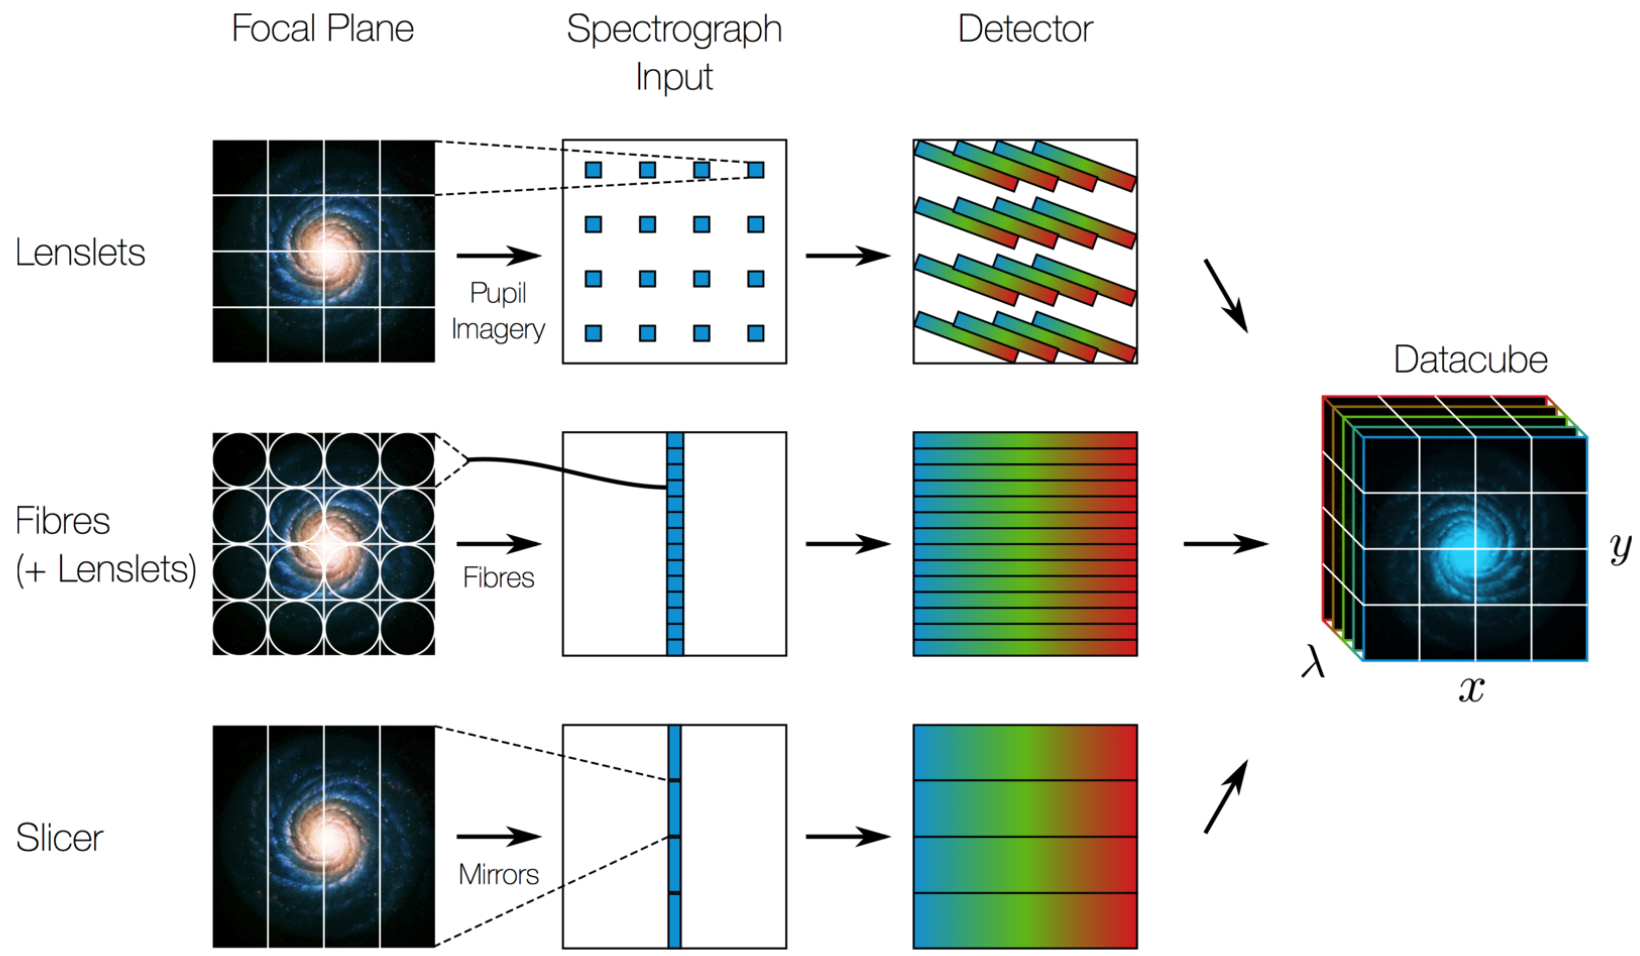
\includegraphics[width=0.9\textwidth]{../figures/03_sedm/ifsgeneral.png}
  \caption[Fonctionnement d'un IFS]{Fonctionnement d'un IFS pour
    différents types d'IFU. La SEDm utilise un système d'agencement de micro-lentilles (cas
    du \textit{haut})
    (\textit{Crédit M. Westmoquette, adaptée de \citet{allingtonIFS}})}
  \label{fig:ifsgeneral}
\end{figure}

Les données brutes obtenues à partir d'un IFS sont ainsi sous la forme
de multiples spectres (de plusieurs dizaines à plusieurs milliers)
étalés (la trace) sur le détecteur, chacun ayant pour origine un élément individuel
de l'IFU. Ces éléments sont en quelques sortes des pixels spatiaux, que
l'on contracte communément par le terme de spaxels. La reconstruction du
cube de données se fait en extrayant chaque spectre du détecteur, et en
les réarrangeant dans le même espace géométrique que le plan focal du
télescope (nous détaillerons ce processus dans la section suivante).

\subsection{La SEDm}\label{ssec:sedm}

Focalisons nous maintenant sur notre instrument, la Spectral Energy
Distribution machine, présenté par \citet{SEDM18}. Comme mentionné plusieurs fois, celui ci est monté
sur le télescope P60 (Cassegrain) au Mont Palomar depuis Août 2016. Une vue
d'ensemble de l'instrument est présenté dans la
Figure~\ref{fig:sedmoverview}, où l'on peut voir qu'il est composé de
deux canaux: l'IFU et la ``Rainbow Camera'' (RC), montés sur un
agencement en forme de T. Cette caméra d'acquisition multi-bande est
accompagnée de 4 filtres photométriques $u'$, $g'$, $r'$ et $i'$.


\begin{figure}[h]
  \centering
  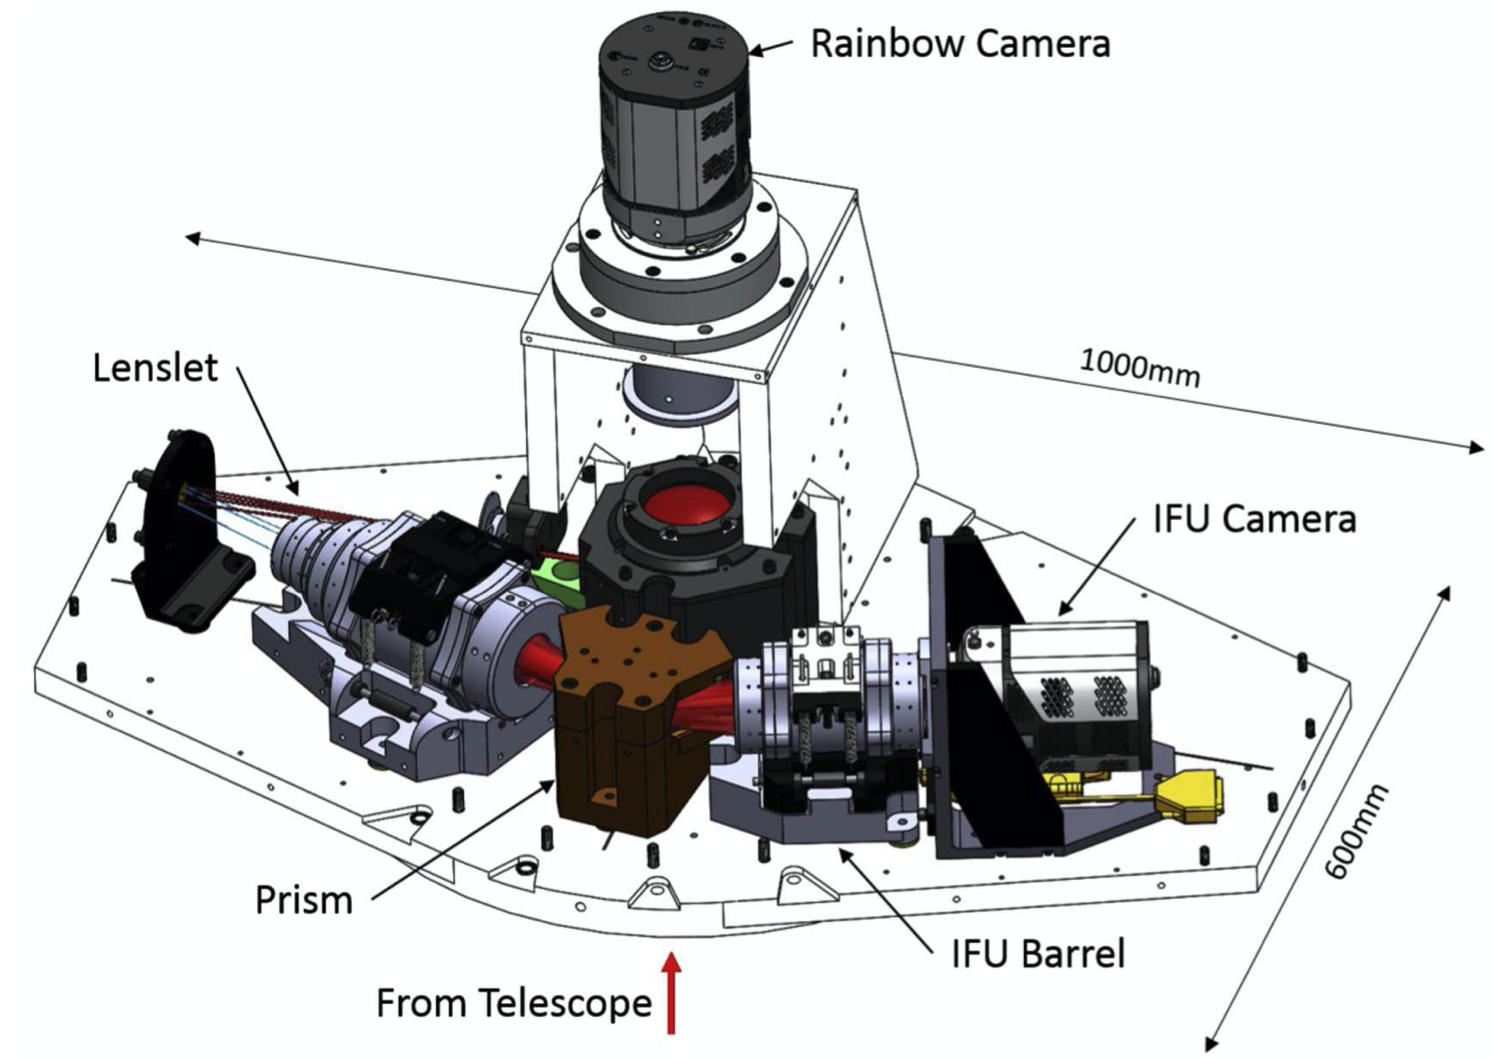
\includegraphics[width=0.9\textwidth]{../figures/03_sedm/sedmoverview.png}
  \caption[Vue d'ensemble de la SEDm]{Vue d'ensemble de la SEDm
    \citep{SEDM18}. La source de lumière du Cassegrain est indiqué par
    la lumière rouge. L'instrument photométrique, la RC, est situé en
    haut au centre et récolte directement la lumière. Pour l'IFU, la
    lumière est redirigée jusqu'à un miroir que l'on peut voir tout à
    gauche de la représentation. Elle est ensuite réfléchie dans le MLA
    (Lenslet). La lumière de chaque micro-lentille du MLA passe ensuite
    dans le prisme (en marron au centre) pour y être dispersé et
    focalisé par l'optique (IFU Barrel) sur le détecteur (IFU Camera).}
  \label{fig:sedmoverview}
\end{figure}

Les 2 caméras de la SEDm sont des Princeton Instruments identiques:
une PIXIS 2048B et une PIXIS 2048B\_Excelon chacun avec 2048$\times$2048
pixels de taille \SI{13.5}{\micro\metre}.

La Rainbow Camera est utilisée pour le guidage, la calibration,
l'acquisition de cible ou encore l'imagerie scientifique. Le champ de
vue de $13\arcmin\times13\arcmin$ est divisé en 4 quadrants, un pour
chacun des filtres $u'g'r'i'$.

L'IFU de la SEDm fonctionne sur la méthode du réseau de micro-lentilles,
le MLA. Celui ci couvre un champ de vue de $28\times28\arcsec$, avec
$45\times52$ lentilles hexagonales. Le faisceau de lumière projeté par
ces lentilles passe dans un triple prisme avec une résolution spectrale
achromatique de $R=\frac{\lambda}{\Delta\lambda}\sim100$.
Comme illustré dans la Figure~\ref{fig:sedmoverview}, c'est la RC qui
est alignée avec la lumière directe en provenance du Cassegrain. Il faut donc en dévier une
partie qui sera transmise à la caméra de l'IFU: cela est effectué avec un
prisme d'interception centré sur le faisceau incident, qui va rediriger
le champ de $28\times28\arcsec$ vers un miroir. Les images
photométriques de la RC ont donc en leur centre un masque qui correspond
au champ de vue de l'IFU. Ainsi pour faire l'acquisition d'une cible
avec l'IFU, il faut d'abord effectuer une acquisition avec la RC sur
laquelle un fitter d'astrometrie est appliqué. Cette étape fournie une
information précise sur le pointage du télescope, et permet donc
d'appliquer l'offset nécessaire pour positionner la cible au centre du
champ de vue de l'IFU.

\section{Extraction des spectres du CCD et création des cubes de données}
\label{sec:pysedmcube}

Dans cette section nous allons détailler la procédure et le pipeline
associé permettant de reconstruire les cubes de données à partir des
images bruts 2D obtenues sur le CCD de l'IFU. Ce passage 2D
$\rightarrow$ 3D nécessite d'identifier 3 éléments:

\begin{minipage}{\linewidth}
\begin{itemize}[label=$\diamondsuit$]
  \itemsep0em 
   \item La localisation de la lumière des spaxels sur le CCD: la trace.
   \item La correspondance entre la localisation de la trace sur le CCD et
     la position du spaxel dans le plan focal.
   \item La cartographie de la dispersion spectral qui permet de
     convertir chaque pixel du CCD en longueur d'onde (et vice versa).
\end{itemize}
\end{minipage}
\vspace{0.1cm}

Ces trois étapes de calibration sont
effectuées durant l'après-midi afin d'optimiser le temps
d'observation. Durant les acquisitions scientifiques, certaines corrections que nous
aborderons plus loin sont effectuées en temps réels.

Toute cette démarche a été implémenté dans le pipeline public
\pysedm\footnote{\url{https://github.com/MickaelRigault/pysedm}}, conçu
par \citet{pysedm} et la suite de cette section résumera une grande partie de cette
publication.
\subsection{Identification des traces}\label{ssec:tracematch}
Commençons par l'identification des traces sur le CCD. Pour cette
étape on effectue une exposition du dome qui sera l'équivalent d'un flat 3D
pour la calibration de l'IFU (les dark et les bias sont directement
corrigés sur les images du CCD).
\vspace{0.1cm}

%\noindent\makebox[\textwidth][c]{%
%  \begin{minipage}{0.99\textwidth}
%    \scriptsize
    \begin{frshaded*}
    \footnotesize
      \centerline{Rappel des images de calibrations.}
      \begin{itemize}
      \item \textbf{Le flat} correspond à une
        aquisition d'une lumière uniforme, ce qui permet de mesurer la réponse
        relative de chaque
        pixel d'un détecteur. En divisant les images de science par ce flat,
        on uniformise alors la réponse de chaque pixel, ce qui permet de
        corriger d'éventuels effets de vignétage (habituellement dominant sur
        les bords du détecteur). Pour le mesurer, il faut illuminer le
        détecteur avec une lumière uniforme. 
        
      \item \textbf{Le dark} lui permet de corriger le bruit dû aux longues
        expositions. Une caméra CCD (ou un capteur CMOS comme dans les
        Reflex) génère un bruit thermique, dont l'intensité dépend de la
        température, du temps de pose et des ISO. Pour diminuer ce bruit, on soustrait le dark aux images de
        science. On créé les dark dans les mêmes conditions que les
        observations (temps d'exposition, température, ISO etc). Ces images sont
        prises dans le noir, avec un couvercle devant
        l'objectif ou un obturateur devant la caméra par exemple.
        
      \item \textbf{Le bias} va quant à lui corriger le bruit inhérent à la
        caméra: le bruit de lecture. Tout comme le dark, il se soustrait
        aux images de science. Tout comme le dark, ces images ce fond
        dans le noir, mais avec le temps d'exposition minimal
        atteignable par la caméra.

      \item \textbf{Le dark-flat} est comme le dark, mais pour les
        images flat.
    \end{itemize}
    Pour chaque type d'image, on procède à l'acquisition d'un certain
    nombre que l'on combine pour former les Master images (Master bias,
    Master dark etc).
    \begin{center}
      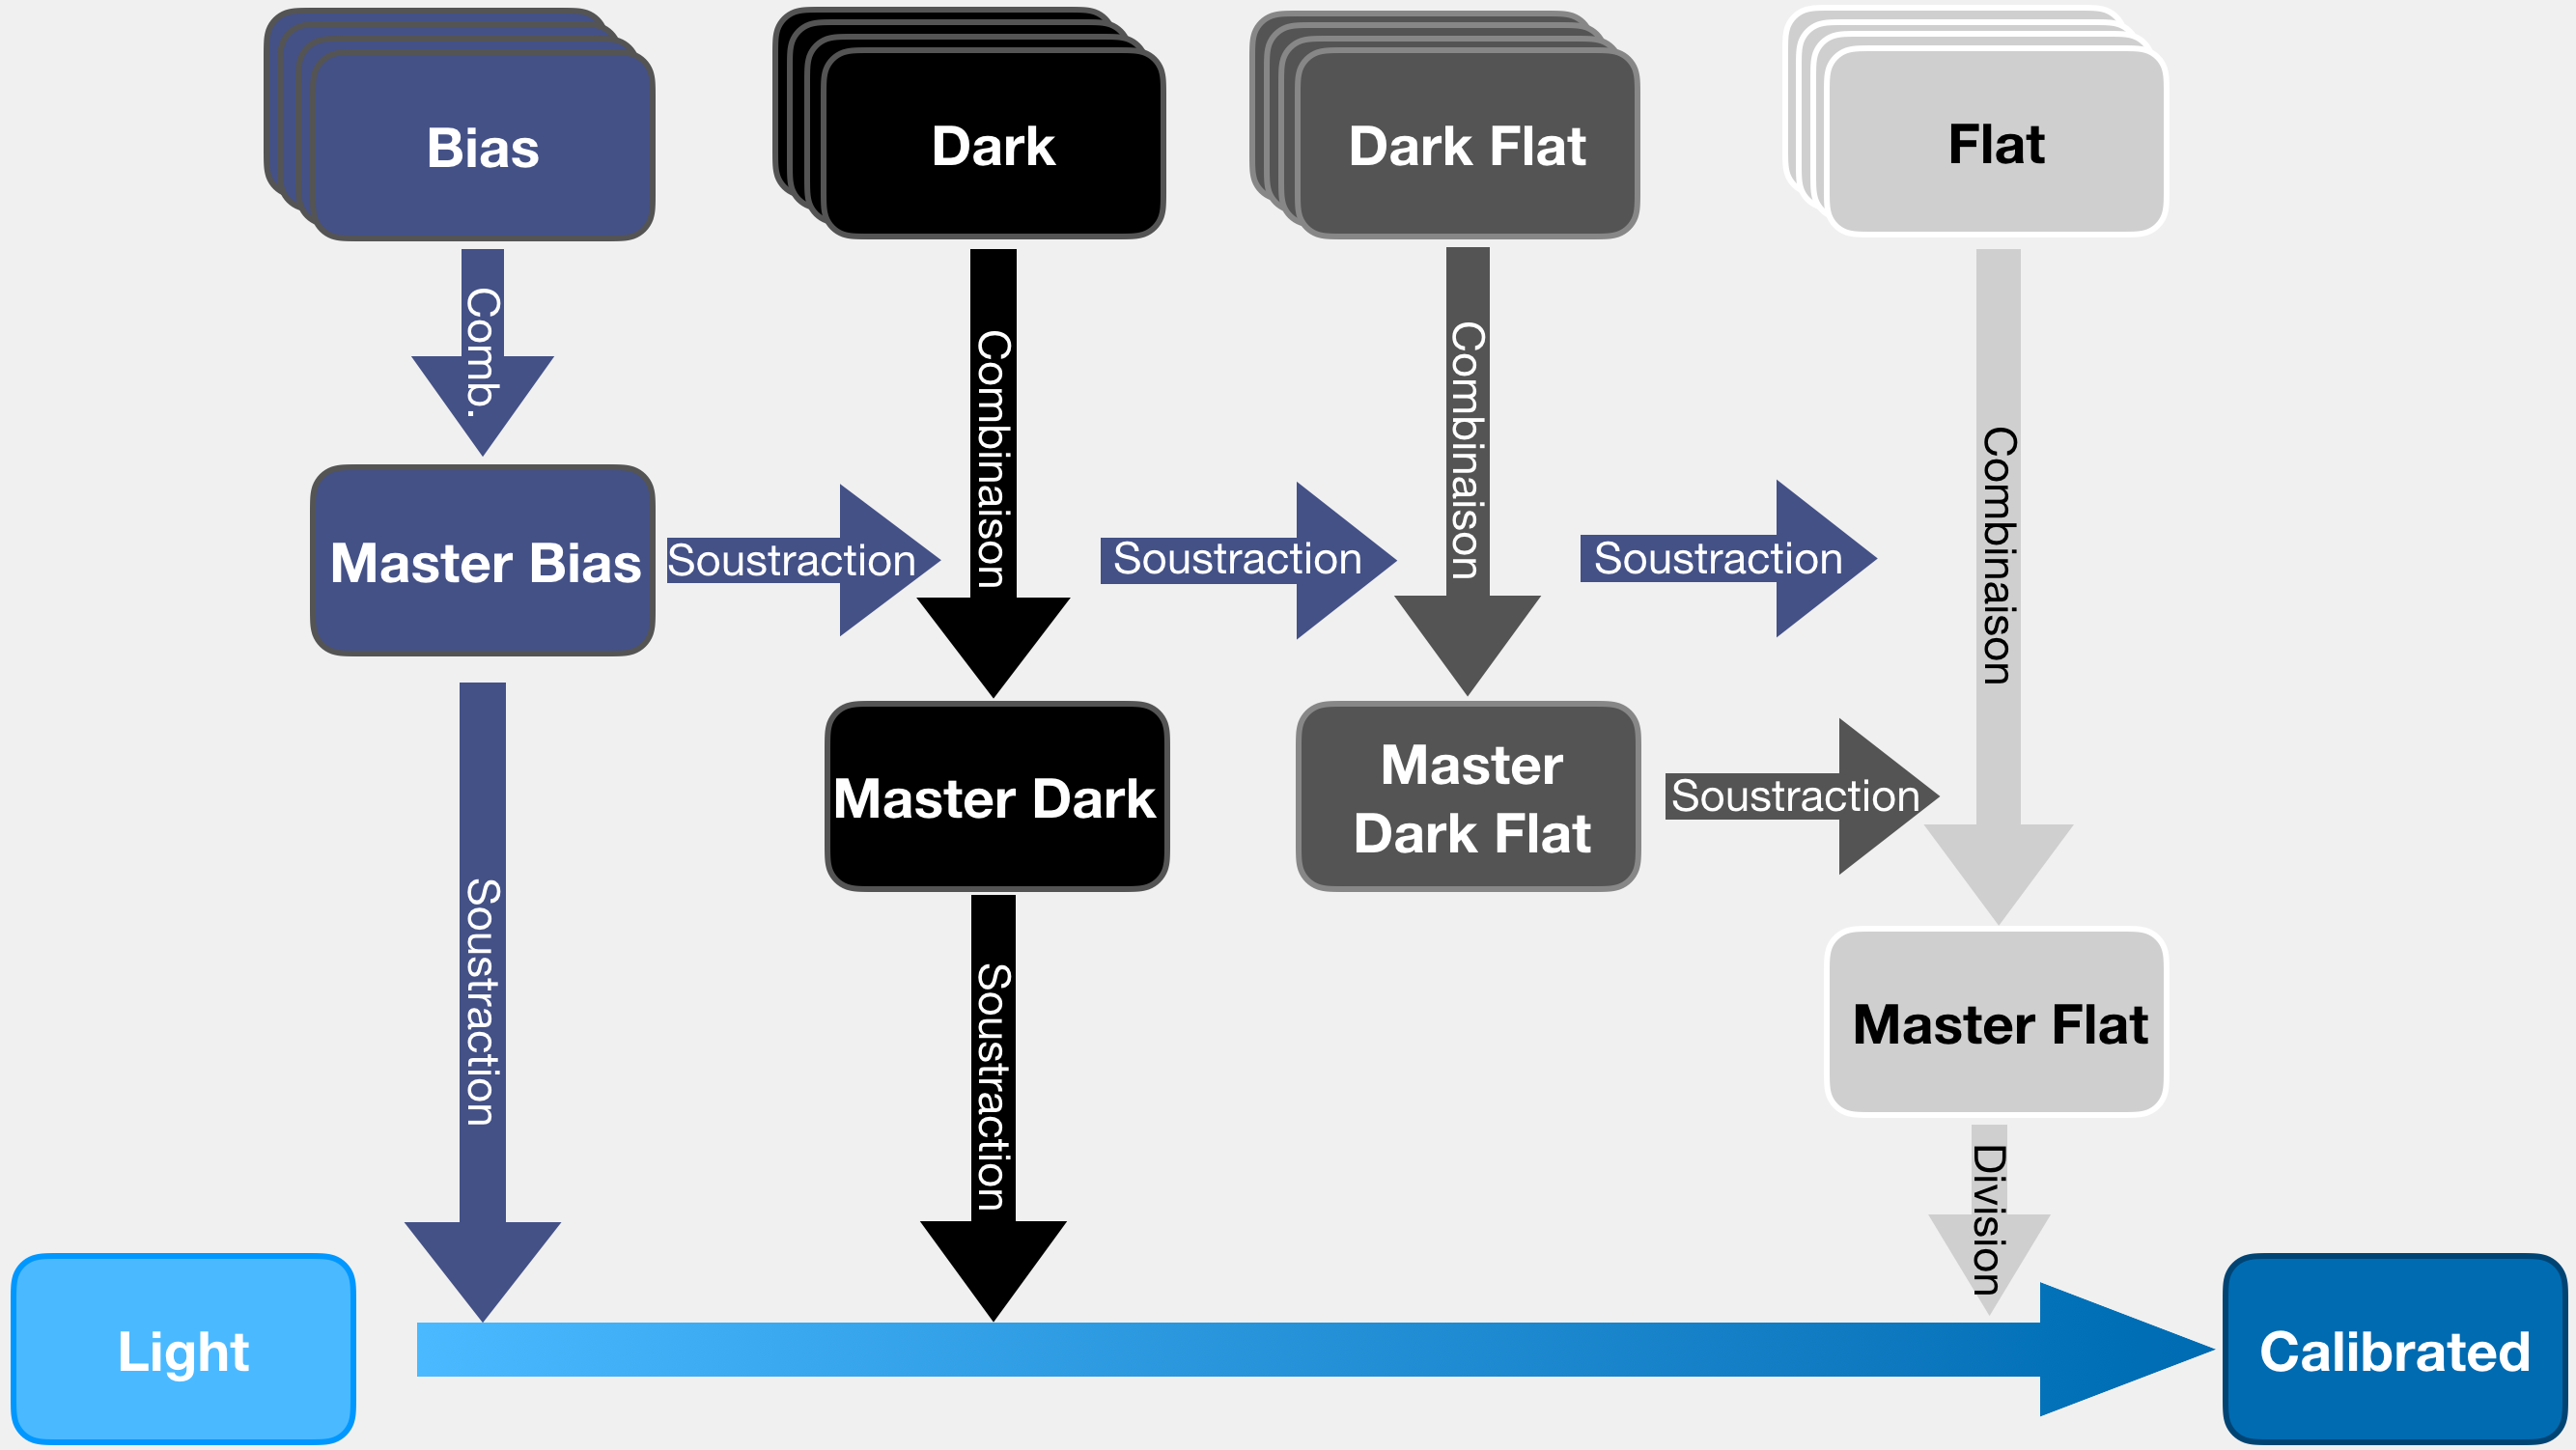
\includegraphics[width=0.8\textwidth]{../figures/03_sedm/calibdag.png}
      \captionsetup{font=footnotesize}
    \captionof{figure}{Schéma d'application d'images de calibration Bias, Dark et Flat}
    \end{center}
  \end{frshaded*}
%\end{minipage}}

Une exposition CCD du dome est représentée dans la
Figure~\ref{fig:tracematch}. L'isolation de la lumière dispersée par
chaque spaxel se fait en définissant une ellipse
via la méthode \pkg{extract} de
\pkg{sep}\footnote{\url{http://github.com/kbarbary/sep}}
\citep{Barbary2016Sep} (implémentation python de \pkg{Sextractor}
\cite{Bertinsextractor}). La trace des spaxels est ensuite isolée en
considérant un rectangle à partir des informations de l'ellipse, de
sorte que $95.5\%$ de la lumière soit encapsulée. L'intervalle de
longueur d'onde ainsi isolé va de $3500$ à $\SI{9500}{\angstrom}$,
respectivement de droite vers la gauche. Un masque 2D pondéré est
ensuite créé prenant en compte la fraction de l'aire de chaque pixel
présent dans le contour défini de la trace. Un spectre pour chaque
spaxel est ainsi extrait en unité de ``count'' par pixel.

\subsection{Solution en longueur d'onde}\label{ssec:wavesol}
On passe maintenant à l'étape qui va permettre d'associer pour chaque pixel une
longueur d'onde, et ce pour chaque spaxel indépendamment.
Pour cette calibration, on utilise 3 lampes à arc qui émettent de fortes
raies d'emissions à des longueurs d'onde connues:

\begin{description}[itemsep=0em]
\item[Hg] Lampe à mercure avec 4 raies d'émission.
\item[Cd] Lampe à cadmium avec 4 raies d'émission.
\item[Xe] Lampe à xenon avec 6 raies d'émission.
\end{description}

La procédure est la suivante (et illustré dans la Figure~\ref{fig:wavesol}):
\begin{enumerate}[(a)]
\item Exposition du CCD pour chaque lampe à arc.
\item Extraction du spectre de chaque spaxel (en unité de pixel) pour chaque exposition.
\item Fit indépendant pour chaque spaxel et pour chaque
  lampe. Pour cela un continuum polynomial de $3\ieme$ ordre est
  utilisé associé à une combinaison de Gaussiennes (autant qu'il y a de
  raies d'émission).
\item Fit conjoint des $14$ centroids des raies d'émission en fonction de
  leur longueur d'onde attendue. Un polynome de degré 5 est utilisé pour
  cette étape.
\end{enumerate}

La précision atteinte pour la solution en longueur d'onde est de l'ordre
de $3$\AA\ au centre de l'IFU, mais peut monter à $\sim10$\AA\ sur les bords.

\begin{figure}[ht]
\centering
\subfloat[Extraction des contours de trace]{\label{fig:tracematch}{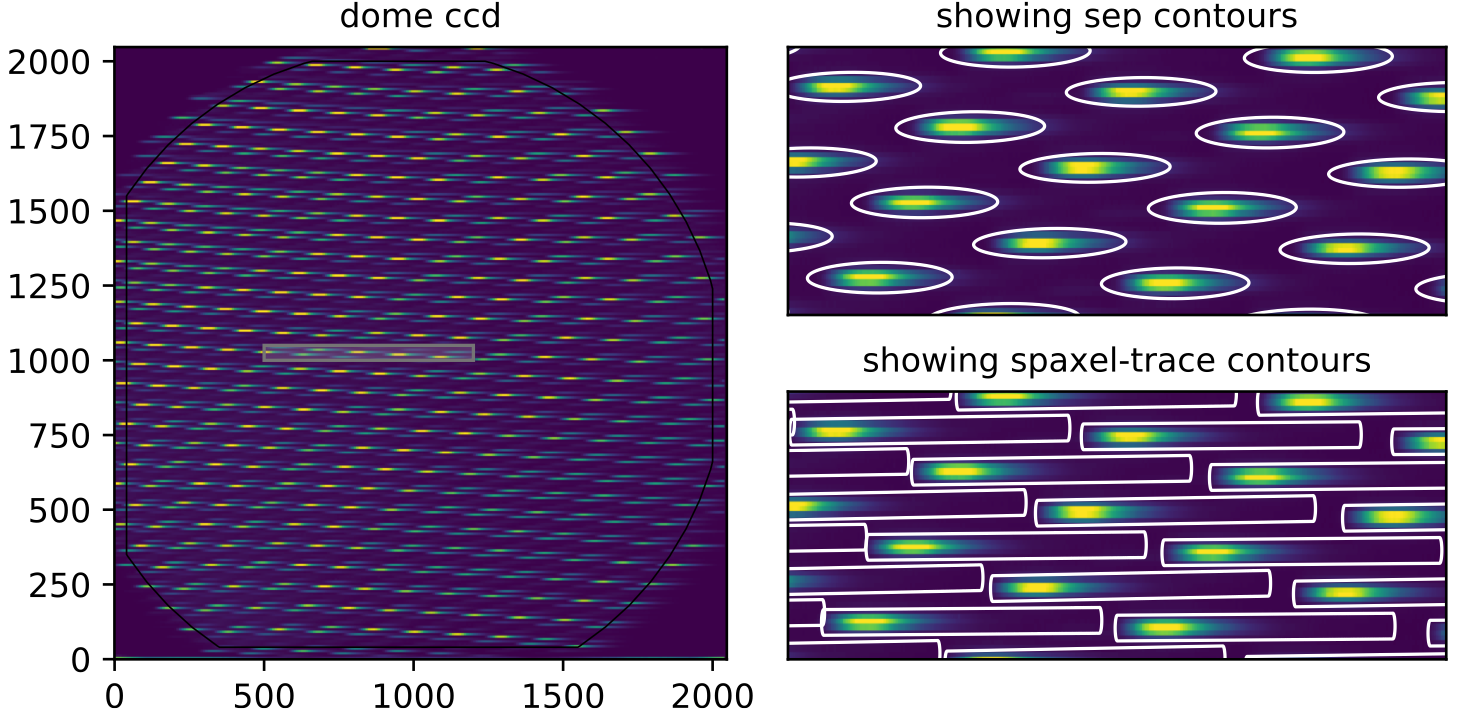
\includegraphics[width=0.53\textwidth]{../figures/03_sedm/tracematchsedm.png}}}\hfill
\subfloat[Fit d'une solution de longueur d'onde pour un spaxel de l'IFU]{\label{fig:wavesol}{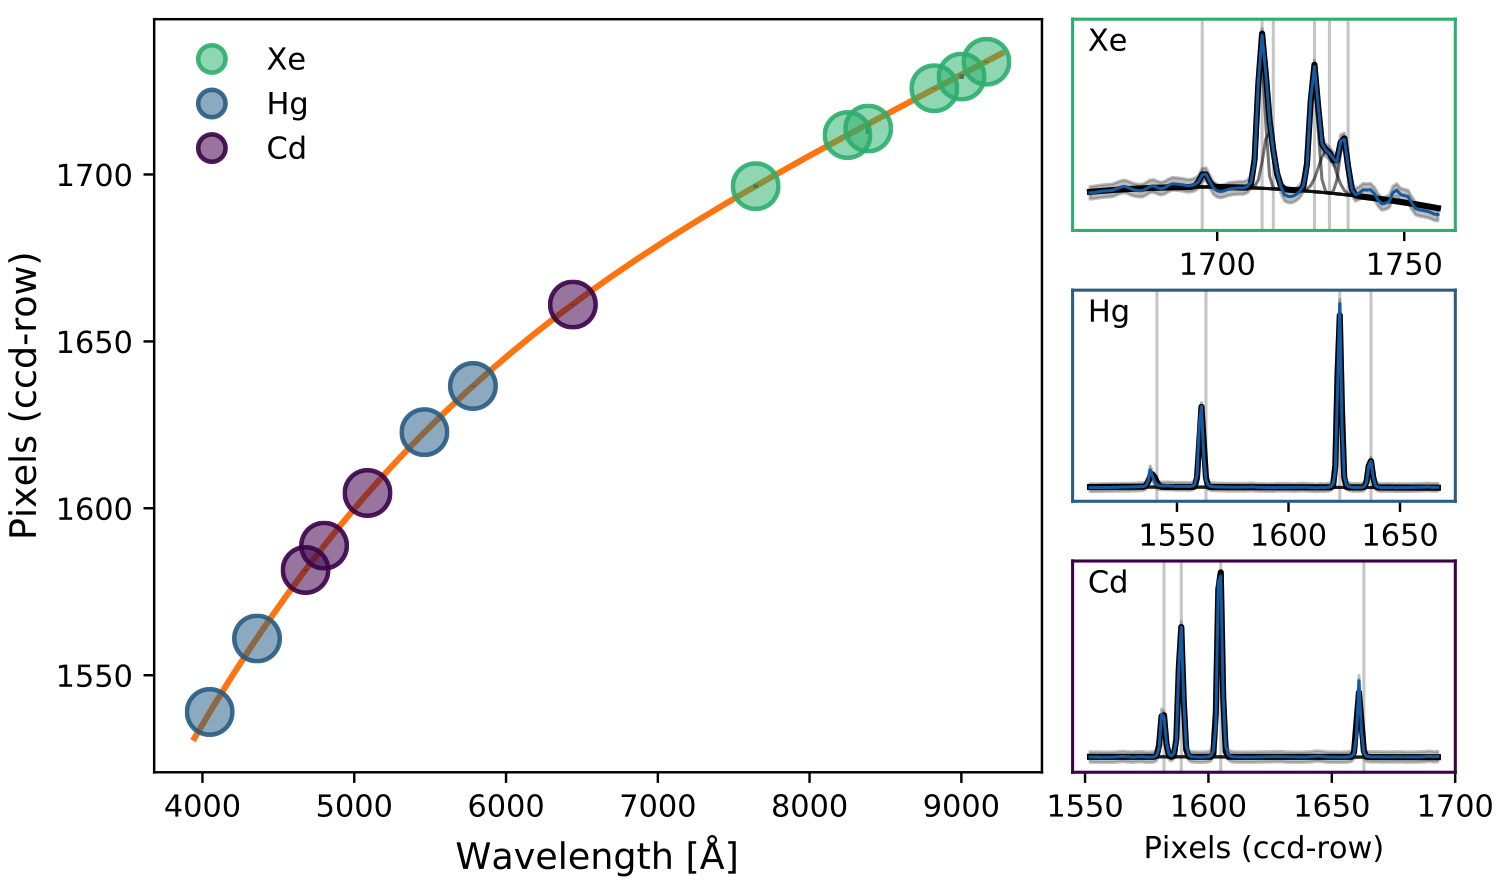
\includegraphics[width=0.45\textwidth]{../figures/03_sedm/wavesolsedm.png}}}
\caption[Extraction de traces et solution en longueur
d'onde pour la
SEDm]{Extraction de traces (\textit{à gauche}) et fit de solution en longueur
  d'onde (\textit{à droite}) pour la SEDm
  (de \citet{pysedm})}
\label{fig:calibsedm}
\end{figure}

\subsection{Identification spatiale}\label{ssec:spaceid}
La dernière étape avant la construction du cube est l'identification
spatiale, afin de récupérer la structure hexagonale du réseau de micro
lentilles.
Cette procédure est purement géométrique et est détaillée en 8 étapes
dans la section 2.1.3 de \citet{pysedm}. Le résultat final est une
grille hexagonale, avec pour chaque hexagone un identifiant associé au
spaxel correspondant ainsi que les coordonnées de chaque vertex.
Combinés aux spectres extraits de chaque spaxel, cela permet de
cartographier la position de chaque spaxel, et ainsi reconstruire le
MLA.

\subsection{Construction du cube 3D}\label{ssec:3dcubecons}
Vient enfin la reconstruction d'un cube après une acquisition
scientifique. Comme expliqué au début de ce chapitre,
toutes les observations d'une nuit sont calibrées 
à partir des informations de calibrations faites durant l'après-midi
(bias, dark, flat, solution en longueur d'onde, localisation de trace
etc).
Cependant certains de ces paramètres peuvent varier au cours de la nuit,
c'est pourquoi 2 étapes de corrections sont appliquées à chaque nouvelle
exposition: Une pour la localisation des traces, l'autre pour la
solution en longueur d'onde. Voici les étapes principales de
reconstruction d'un cube 3D à partir d'une image 2D du CCD (on ne
détaillera pas ici chacune des étapes mais nous invitons le lecteur à
consulter \citet{pysedm} pour plus d'information technique):

\begin{enumerate}[(a)]
\itemsep=0em
\item Optimisation de la localisation des traces en effectuant une
  correction verticale de l'ensemble du réseau.
\item Soustraction du background du CCD, construit à partir des pixels
  qui sont en dehors des traces. 
\item Extraction des spectres en unité de coups par pixel, projection dans
  l'espace des longueur d'onde grâce à la solution en longueur d'onde,
  puis création du cube grâce à l'identification spatiale des spaxels.
\item Estimation de la déviation en longueur d'onde en mesurant les
  raies telluriques et du ciel (connues). Cette correction
  $\Delta\lambda$ est ensuite convertie en une correction horizontale
  $\Delta i$ de pixel.
\item Répétition de l'étape (c) en corrigeant de la déviation $\Delta i$
  mesurée dans (d) lors du passage de l'espace des pixels vers l'espace
  des longueur d'onde.
\item Application du cube Flat (exposition du dome) pour corriger la réponse relative des spaxels.
\end{enumerate}

\section{Actuelle méthode d'extraction de source ponctuelle}
\label{ssec:pysedmextractstar}

\subsection{Localisation de la cible}\label{ssec:targetlocpysedm}

Avant d'extraire la source ponctuelle ciblée avec l'IFU, encore faut-il
pouvoir la localiser dans le MLA.

Le faible champ de vue de l'IFU de la SEDm ne permet habituellement pas
d'observer simultanément de nombreuses sources. En générale, seule la
cible et sa galaxie hôte sont visibles dans la MLA, ce qui ne permet pas
d'en résoudre la solution astrométrique.

Une première option triviale est de la
localiser manuellement. Mais l'automatisation de cette étape est bien
entendue privilégiée. Dans le cas de l'observation d'une étoile standard isolée
(pour la calibration photométrique), il est suffisant d'estimer sa
position à partir des spaxels les plus brillants (ou la médiane de la
position de N spaxels pour éviter un outlier comme un rayon cosmique).

Mais dans le cas de l'observation d'un transient, c'est un peu plus
subtil. Cette dernière peut en effet être accompagnée de sa galaxie hôte
dans le champ de vue, et la méthode des spaxels brillants ne marche en
générale plus.

Nous avons mentionné dans la section~\ref{ssec:sedm} que la SEDm était,
en plus de l'IFU, équippée d'une Rainbow Camera, un canal
photométrique avec un champ de vue bien plus important de
$13\arcmin\times13\arcmin$. Le prisme d'interseption pour l'IFU étant
fixé, il est possible de déterminer une solution WCS (World Coordinate
System) à partir des images de guidage, et de les projeter dans le MLA à
une longueur d'onde de référence arbitraire. La solution WCS permet
ainsi de passer de l'espace des pixels/spaxels à l'espace des
coordonnées célestes \textit{et vice versa}. Connaissant la position
céleste de la cible (par détection photométrique avec la
caméra ZTF), on peut ainsi déterminer sa position dans le MLA. Cette
méthode est précise à environ $1-2\arcsec$ près.

\subsection{Extraction de la source ponctuelle}\label{ssec:sourceextractpysedm}

Une fois la position de la cible connue, on peut à présent en extraire
le spectre du cube de données. La première étape est de modéliser la
source ponctuelle, qui est entièrement définie par sa position, sa fonction
d'étalement de point (PSF), et son amplitude. Il faut à cela
rajouter une composante de fond, le background, qui doit modéliser le
ciel (constante) mais également la lumière de la galaxie hôte, considéré ici
comme un background structuré.

Le processus d'extraction est la scission du cube 3D en N$\times$2D
meta-tranches indépendantes (1 meta-tranche étant un empilement de $n$
tranches pour un meilleur ratio signal/bruit), l'extraction de la source ponctuelle dans chacune
d'elles, et enfin l'extrapolation à tout le cube en modélisant la
chromaticité.
Dans un premier temps le pipeline \pysedm considère un disque de rayon $10$
spaxels autour de la position de la cible estimée avec les images de
guidage (section~\ref{ssec:targetlocpysedm}). Cette position est une
condition initiale, et permet de se limiter à un sous-cube (un cylindre
de rayon $10$ spaxels).

Raisonnons en 2D. Dans chaque meta-tranche nous avons à déterminer:
\begin{itemize}[label=$\bullet$]
\itemsep0em 
\item \textbf{Le background}, qui est structuré à cause de la
  présence potentielle de la galaxie hôte dans le champ de vue, est
  modélisé par un polynome d'ordre $2$, et a ainsi $3$ paramètres libres. 
\item \textbf{L'amplitude} de la source ponctuelle, $1$ paramètre libre.
\item \textbf{La position} ($x$, $y$) de la source ponctuelle, $2$ paramètres libres.
\item \textbf{La PSF} de la source ponctuelle, modélisée par une
  combinaison linaire Gaussienne + Moffat (\citet{Butonthese},
  \citet{Buton2013}). Ce modèle est paramétré avec $3$ paramètres libres
  dans \citet{pysedm}: le rayon de la Moffat, celui de la Gaussienne et
  le poids entre les deux distributions. Il faut également rajouter $2$ paramètres libres
  d'ellipticité (un pour l'angle, l'autre pour l'excentricité).
\end{itemize}

Tous ces paramètres sont fittés pour chaque meta-tranches prises
indépendamment les unes des autres.

Le set de paramètres ainsi obtenu est utilisé pour déterminer la
chromaticité de la position et de la PSF. L'amplitude et
le background sont des paramètres de nuisance à ce stade.
Dans \pysedm, la chromaticité de l'ellipticité, du rayon de la Moffat et du poids entre la
Gaussienne et la Moffat sont modélisés par une constante. La
chromaticité du rayon de la
Gaussienne est modélisé par une loi de puissance.
Quant à la position, sa chromaticité est due à la réfraction de la
lumière par l'atmosphère. C'est ce qu'on appelle l'ADR (Atmospheric
Differential Refraction). Nous détaillerons en détail cet effet et sa
modélisation dans la
Partie II de ce manuscrit (Section~\ref{ssec:chromadr}).
Ainsi, les paramètres des modèles de chromaticités sont à leur tour
fittés à partir du set de paramètres obtenu avec les N$\times$2D
meta-tranches.

Une fois cela effectué, la PSF et la position de la cible sont fixées pour
chaque longueur d'onde, et un dernier fit linéaire sur l'ensemble du
cube est effectué pour les
paramètres du background et de l'amplitude de la PSF. L'extraction de
cette amplitude à chaque longueur d'onde du cube de données fournit
ainsi le spectre de la source ponctuelle.


\subsection{Calibration en flux}\label{ssec:calibpysedm}

Le spectre extrait dans la section~\ref{ssec:sourceextractpysedm} étant en
unité de pseudo-ADU (Analog to Digital Units), il faut à présent procéder à sa
calibration afin de pouvoir l'exprimer en unité de flux physique.
Le spectre d'une source astronomique observée peut être exprimé suivant
le formalisme suivant \citep{Buton2013}:
\begin{equation}
  \label{eq:calibbutoon}
  S(\lambda,t,z)=S^{\star}(\lambda,t)\times\mathcal{C}(\lambda,t)\times T_{atm}(\lambda,t,z)
\end{equation}
Avec $S^{\star}(\lambda,t)$ le spectre instrinsèque de la source en
unités physiques ($erg/cm^2/s/$\AA), $\mathcal{C}(\lambda,t)$ la réponse
instrumentale, et $T_{atm}(\lambda,t,z)$ la transmission atmosphérique, qui
dépend de la masse d'air le long de la ligne de visée. Calibrer un
spectre revient donc à déterminer $\mathcal{C}$ et $T_{atm}$ pour isoler $S^{\star}$.

En toute rigueur, la transmission atmosphérique devrait être décomposée
en composantes physiques bien connues comme la diffusion de Rayleigh, la
diffusion aérosol,
l'absorption de l'ozone et l'absoption telluriques
(\citet{Hayes1975atm}, \citet{Wade1988atm}, \citet{Stubbs2007atm} ).

Dans le cadre de la SEDm, le but n'étant pas de faire une étude
spectrophotométrique des sources observées, ce formalisme a été
fortement simplifié et est exprimé tel que:

\begin{equation}
  \label{eq:calibbutoon}
  S(\lambda,t,z)=S^{\star}(\lambda,t)\times\left[\mathcal{C}(\lambda,t)+\mathcal{ T}(\lambda,t,z)\right]
\end{equation}

Où $\mathcal{ T}$ représente l'absoption tellurique. Les spectres
telluriques utilisées sont ceux du Kitt Peak National
Observatory\footnote{\url{http://www.noao.edu/kpno/}} \citep{Hinkle2003}, scindés en deux
catégories de longueur d'onde: l'$\text{O}_{2}$ et
l'$\text{H}_{2}\text{O}$.
L'absoption tellurique est alors exprimée suivant:

\begin{equation}
  \label{eq:telluricpysedm}
  \mathcal{T}(z) =
  \mathcal{T}_{\text{O}_{2}}\times(c_{\text{O}_{2}}+z^{\rho_{\text{O}_{2}}})
  + \mathcal{T}_{\text{H}_{2}\text{O}}\times(c_{\text{H}_{2}\text{O}}+z^{\rho_{\text{H}_{2}\text{O}}})
\end{equation}
Où les amplitudes relatives $c_{i}$ et les dépendances en masse d'air
$\rho_{i}$ sont des paramètres libres. Quant à la réponse instrumentale
$\mathcal{C}$, elle est modélisée par un polynome de Legendre d'ordre $20$.

La détermination des composantes $\mathcal{C}$ et $\mathcal{T}$ est alors la suivante:

\begin{enumerate}[(a)]
  \itemsep=0em
\item On observe des étoiles standard du catalogue Calspec
  \citep{Bohlinstdcalpsec} avec la SEDm.
\item On en extrait le spectre en pseudo-ADU avec la méthode
  d'extraction de source ponctuelle
  (Section~\ref{ssec:sourceextractpysedm}).
\item On récupère dans les archives calspec\footnote{\url{https://archive.stsci.edu/hlsps/reference-atlases/cdbs/current_calspec/}} le spectre
  spectrophotométrique correspondant à l'étoile standard observée.
\item Les composantes de réponse instrumentale $\mathcal{C}$ et
  d'absoption telluriques $\mathcal{T}$ sont fittées simultanément en
  minimisant la quantité ~$(S_{ADU}/S_{ref}) - (\mathcal{C} + \mathcal{T})$.
\end{enumerate}

Au moins une étoile standard est observée chaque nuit. La calibration
d'une observation scientifique se fait en considérant la masse d'air
associée (l'absorption tellurique est airmass-dépendante). On obtient
alors le spectre calibré simplement en effectuant l'opération:
\begin{equation*}
  S^{\star}(\lambda,t,z)=\frac{S_{ADU}(\lambda,t)}{\mathcal{C}(\lambda,t)+\mathcal{T}(\lambda,t,z)}
\end{equation*}

On appelle la quantité $(\mathcal{C} + \mathcal{T})$ la courbe de
sensibilité inverse.
La précision de la calibration en flux des spectres de science acquis
avec la SEDm en utilisant le pipeline \pysedm est de l'ordre de quelques pourcents.

\section{Classification}

Rappelons que le rôle premier de la SEDm au sein de la collaboration ZTF
est la \underline{classification} des évènements transitoires. 

Les deux classifieurs spectraux principaux existants sont \pkg{superfit}
\citep{HowellSuperfit} et \pkg{SNID} \citep{BlondinSNID}. \pkg{superfit}
est un software écrit en \pkg{IDL} utilisant une méthode de
minimisation de $\chi^{2}$, et \pkg{SNID} est quant à lui écrit
en \pkg{fortran} et utilise l'algorithme de corrélation croisée de \citet{TonryDavis}.
Nous pouvons également mentionner le plus récent classifieur de
supernovae \pkg{DASH} \citep{MuthukrishnaDash}, utilisant une approche de deep learning.

Dans le pipeline de réduction de données de la SEDm, c'est le
classifieur \pkg{SNID} qui est utilisé. Ce dernier est disponible publiquement\footnote{\url{https://people.lam.fr/blondin.stephane/software/snid/}} et
régulièrement mis à jour. Pour effectuer l'analyse des corrélations
entre le spectre d'entrée et la base de données, un pré-traitement est
effectué (section 2.3 de \citet{BlondinSNID}). Celui ci consiste en (1) Binner le spectre d'entrée en coordonées
$\ln(\lambda)$, (2) Diviser par le continnum du spectre estimé à partir
d'une spline d'ordre $13$ et enfin (3) Appliquer un filtre passe-bande d'ordre $4$.

La fiabilité de la classification est quantifiée par $2$ paramètres: le
ratio ``hauteur-bruit'' $r$ qui quantifie l'importance du pic de la
fonction de correlation normalisée, et le paramètre de superposition des
spectres (lap), qui est par définition compris entre
$0<\text{lap}<\ln(\lambda_{1}/\lambda_{2})$ (où $\lambda_{1}$ et $\lambda_{2}$
sont les extrema de l'intervalle de longueur d'onde communs entre le
spectre d'entrée et les spectres de la base de données).

Associés, ces deux paramètres forment un paramètre de qualité, le
$r\text{lap}=r\times\text{lap}$. Dans la section 6.1 de
\citet{BlondinSNID}, il est montré qu'avec un $r\text{lap}\gtrsim 5$
la confusion entre une SNIa et un autre type est quasi non-existant
($\lesssim2\%$) sans aucune contrainte sur le resdshift ou la phase de
la supernova.

De ce fait, \pysedm reporte tout spectre classifié quelque soit le type
lorsque le paramètre de qualité $r\text{lap}>5$. Nous présentons dans la
Figure~\ref{fig:pysedmoutput} un exemple d'extraction de source
ponctuelle avec \pysedm et sa classification avec \pkg{SNID}.

La banque de modèles utilisée comme référence pour la classification est
une combinaison de plusieurs set de données:
\begin{itemize}
  \item Le set d'entraînement utilisé par \pkg{DASH}
    \citep{MuthukrishnaDash}: celui-ci est composé du \pkg{template-2.0}
    de \pkg{SNID}, de SNIb/c de \citet{Liu2014SNIbc},
    \citet{Mojdaz2016} et \citet{Liu2016}, ainsi que des spectres du programme SN Ia 7.0
    de Berkeley \citep{Silverman2012}.
  \item Les spectres SNIIP de \citet{GutierrezSNII}.
  \item Les spectres SLSN-Ic de \citet{Liu2017SLSN}.
  \item Plusieurs SLSN-I, SLSN-IIn et TDE ajoutés par J.D.Neill.
\end{itemize}

Les spectres pour lesquels la date du maximum de luminosité ont été
retirés.
La banque de données finale utilisée pour \pkg{SNID} contient 3288 spectres de 312 SNe Ia, 1055 spectres de 80 SNe Ib/c, 620 spectres de 33 SNe II, 207 spectres de 35 SLSNe, 29 spectres de 7 TDE, 15 spectres de 3 LBVs, 11 spectres de 11 galaxies, 11 spectres de M-stars, et 1 spectre de 1 AGN.
\begin{figure}
  
  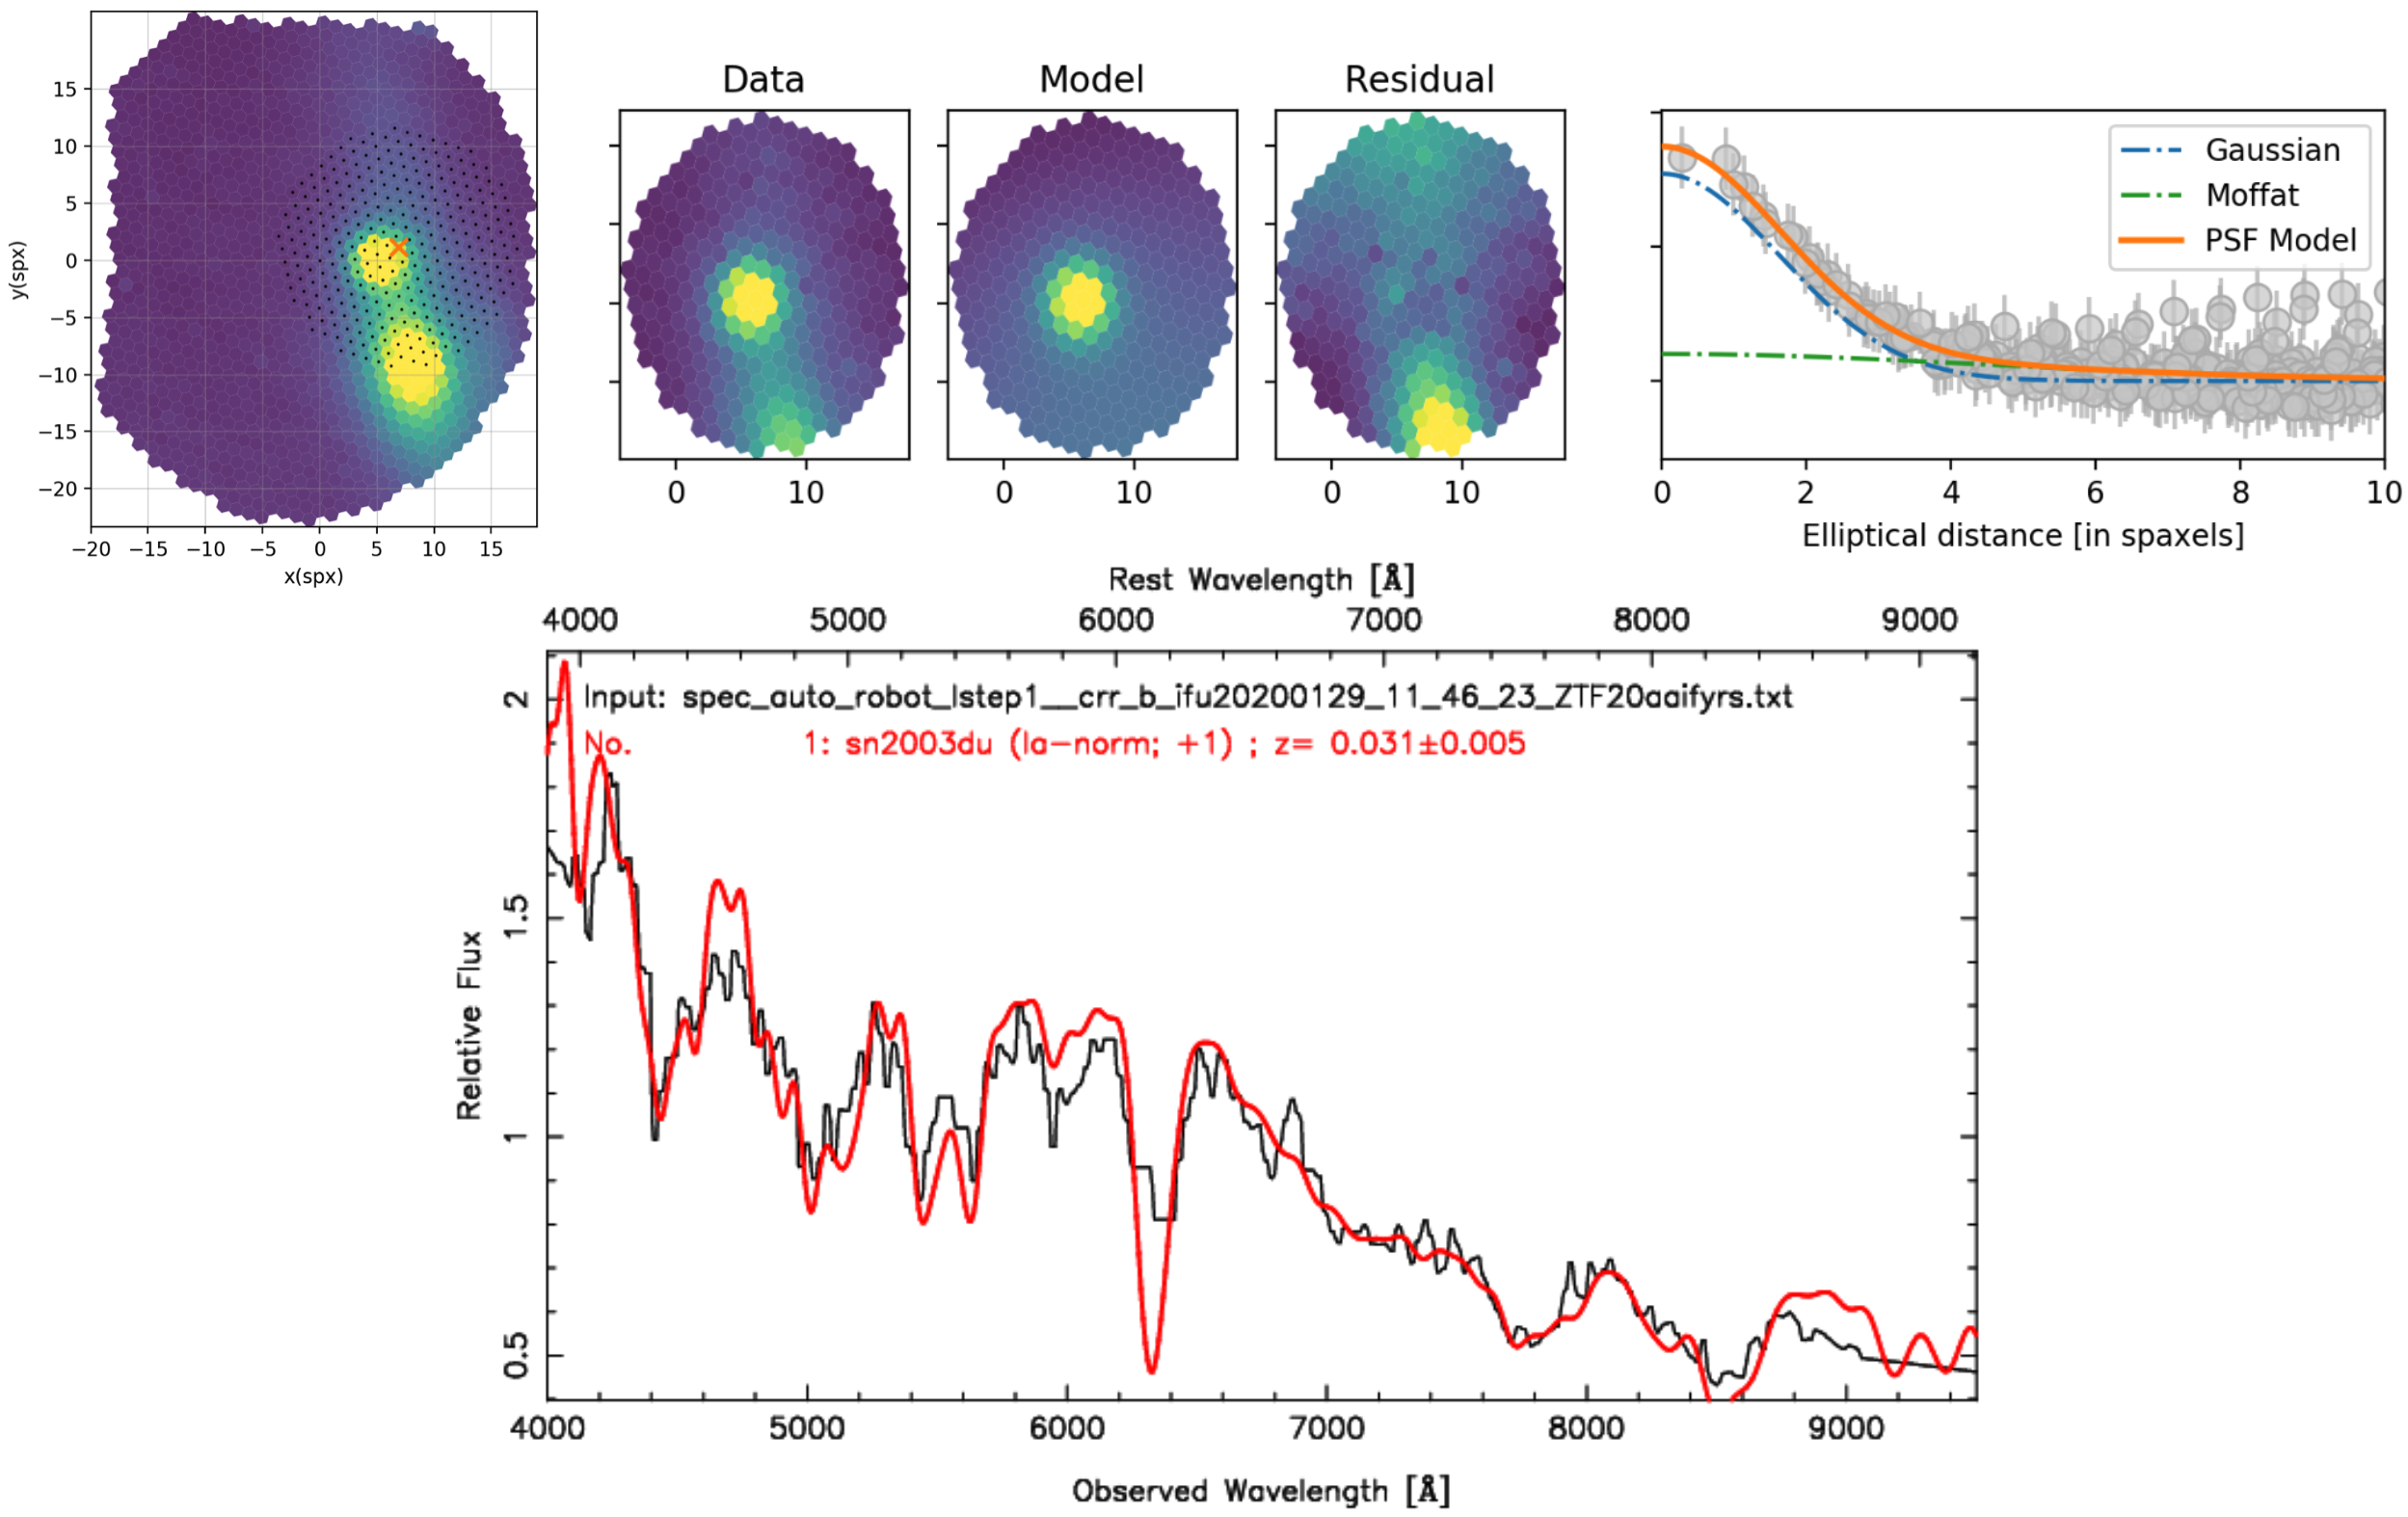
\includegraphics[width=0.99\textwidth]{../figures/03_sedm/pysedmoutput.png}
  \caption[Exemple d'extraction de source ponctuelle avec
  \pysedm]{Exemple d'extraction de source ponctuelle avec \pysedm:
    ZTF20aaifyrs. \textit{En haut, de gauche à droite}: (a) Image 2D intégré
    du cube 3D extrait suivant les étapes de la section~\ref{sec:pysedmcube}. La croix orange indique la position estimée de la source
  ponctuelle à partir des images de guidages de la RC
  (section~\ref{ssec:targetlocpysedm}). Les marqueurs noirs
  correspondent aux spaxels considérés pour l'extraction de la source. (b) Meta-tranche intégrée entre
  $\lambda=[5750-6167]$\AA\, centré sur la position estimée de la source
ponctuelle et de rayon $10$ spaxels. (c) Modèle fitté avec la composante
de background et la PSF (section~\ref{ssec:sourceextractpysedm}). (d)
Résidu Data-Modèle, le signal résiduel en bas correspond à un bout de la
galaxie hôte. (e) Profil radial de la source ponctuelle, exprimé en
pseudo-ADU en fonction du rayon elliptique après soustraction du modèle de background. La courbe bleue
représente la composante Gaussienne, la courbe verte la Moffat et la
courbe orange le profil modélisé total. Les données sont représentées par les
marqueurs gris avec leur barre d'erreur. \textit{En bas}: Spectre
extrait en noir, et le meilleur modèle de supernova fitté par \pkg{SNID}
en rouge. On peut clairement voir ici que la source ponctuelle extraite
est une Supernova de type Ia proche de son pic de luminosité.}
  \label{fig:pysedmoutput}
\end{figure}

\section{Contamination par la galaxie hôte}

Il est indéniable que le pipeline \pysedm, de par sa polyvalence et son
automatisation, est d'une grande efficacité en ce qui concerne la
réduction de données et l'extraction de sources ponctuelles.

Cependant cela n'est rendu possible que lorsque la source ponctuelle est
isolée de sa galaxie hôte dans le champ de vue de l'IFU. Dans le cas
contraire, nous entrons dans un régime de contamination qui nuit à la
qualité de l'extraction, et a fortiori peut empêcher la classification
spectral de la supernova. Sachant que la FWHM d'une source ponctuelle
est de l'ordre de $2\arcsec$ pour la SEDm, il est raisonnable de
considérer une contamination croissante par la galaxie hôte lorsque la
distance angulaire passe en deça des $4\arcsec$, jusqu'à être presque
confondu dans le coeur de la galaxie hôte en deça de $2\arcsec$
(n'oublions pas que le bulbe de la galaxie
est également étendue). Hors nous pouvons voir dans la
Figure~\ref{fig:cumulsnhostdist} \citep{FremlingZTFspec2020}, que près
de $60\%$ des SNeIa sont à une distance angulaire inférieur à
$4\arcsec$, et $40\%$ pour les supernovae à effondrement de coeur. Cette
fraction passe à $45\%$ et $25\%$ en deça de $2\arcsec$ pour les SNeIa
et CC SNe respectivement, et environ $20\%$
et $10\%$ en deça de $1\arcsec$.


\begin{figure}
  \begin{minipage}[c]{0.55\textwidth}
    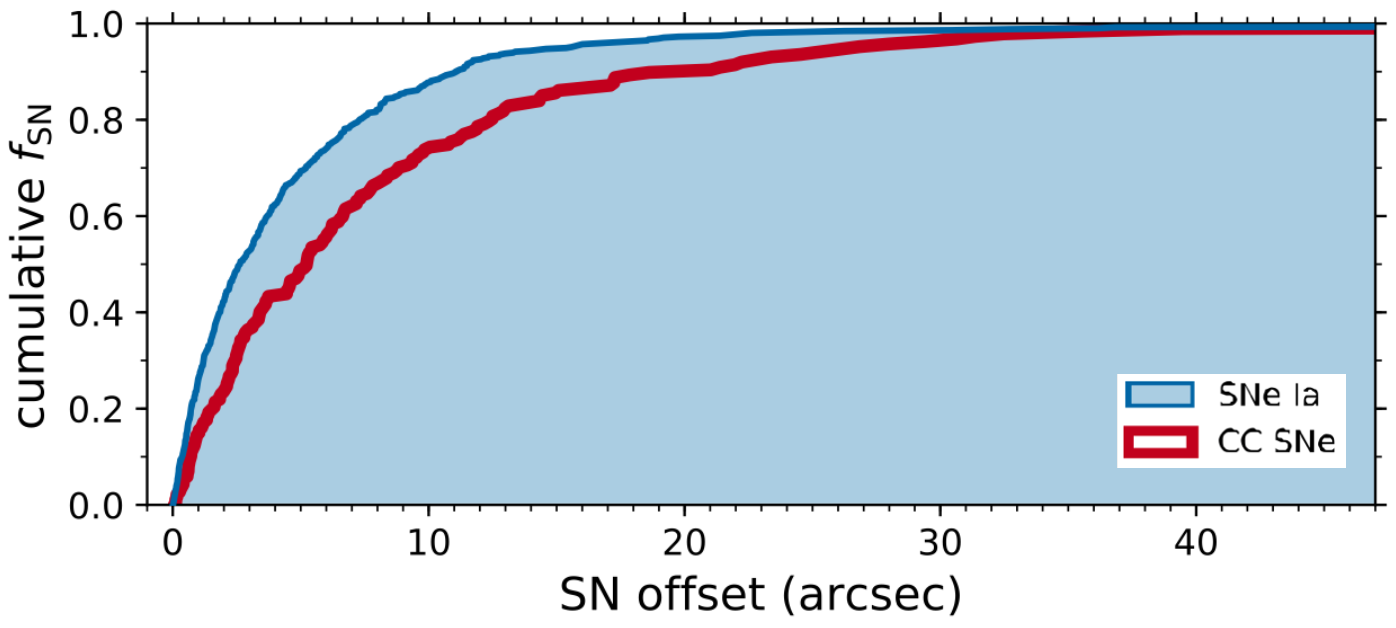
\includegraphics[width=\textwidth]{../figures/03_sedm/cumulsnhostdist.png}
  \end{minipage}\hfill
  \begin{minipage}[c]{0.42\textwidth}
    \caption[Distribution cumulée du décalage angulaire entre les supernovae BTS et leur galaxie hôte]{Distribution cumulée du décalage angulaire, en
    secondes d'arc, entre les supernovae BTS et leur galaxie hôte
    (Figure 6 de \citet{FremlingZTFspec2020}). L'anagramme ``CC'' fait référence au
    terme ``Core-Collapse''. Les supernovae de type Ia ont
  un redshift en moyenne plus élevé, ce qui explique cette
  distribution de plus faible distance angulaire comparé aux autres types.}\label{fig:cumulsnhostdist}
  \end{minipage}
\end{figure}

Dans le cadre d'une observation où la source ponctuelle est faiblement
contaminée par son hôte, une sensible amélioration
de la méthode d'extraction a été apporté par \citet{Kimcontsep} avec ses
modules \pkg{byecr} et \pkg{contsep}:

\begin{itemize}[label=$\bullet$]
\itemsep0em 
\item \textbf{\pkg{BYECR}} a pour rôle de retirer
les rayons cosmiques après construction des cubes de données, afin
d'utiliser les informations spatiales. Ce module va
normaliser le flux de chaque voxel en le divisant par le flux moyen dans
un interval de $[-10,10]$ tranches spectrales. Une
comparaison est ensuite effectué entre le flux du voxel considéré  et celui de ses $6$
(structure hexagonale)
voisins. Un écart supérieur à $5\sigma$ est considéré comme une présence
d'un rayon cosmic, et le voxel en question est ainsi ignoré lors de
l'extraction spectral de la source ponctuelle.
\item \textbf{\pkg{CONSTEP}} Le but ici est de tenter d'ignorer
  automatiquement les spaxels où le flux est dominé par celui de la
  galaxie hôte. L'idée est de trouver le contour d'isomagnitude le moins
  brillant qui sépare la galaxie de la source
  ponctuelle. \citet{Kimcontsep} (Section 2.2 et Figure 2) utilise les images dans
  la bande $r$ du relevé PANSTARRS \citep{ChambersPanstarrs}, dans
  lesquels une source ponctuelle fictive de magnitude $16$ est insérée à
  la position céleste de détection. Cela permet alors de récupérer les
  contours d'isomagnitude, et ainsi ne sélectionner ``que'' les spaxels
  de la source ponctuelle lors de son extraction.
\end{itemize}

Vis à vis du problème de la contamination par la galaxie hôte, seul \pkg{contsep}
est d'intérêt. Seulement, celui ci n'apporte qu'une augmentation de
l'ordre de $0.5\%$ du nombre de spectres classifiés (Table 2 de
\citet{Kimcontsep}), aucun changement notable dans la distribution des
$r\text{lap}$ obtenus avec \pkg{SNID}, et une amélioration globale de la
classifcation de $1.5\%$ en se basant sur celles de l'échantillon BTS comme référence.

En effet, \pkg{contsep} n'apporte (presque) aucun bénéfice dans le cas où
l'astrométrie dans le MLA est peu précise et/ou quand la source ponctuelle n'est pas
séparée du coeur de la galaxie hôte.

La Figure~\ref{fig:stronghost} illustre une telle situation, dans un cas
extrême où la supernova (ici ZTF19acbjlnt) explose quasiment dans la ligne de visée du
coeur de la galaxie.

\begin{figure}
  \centering
  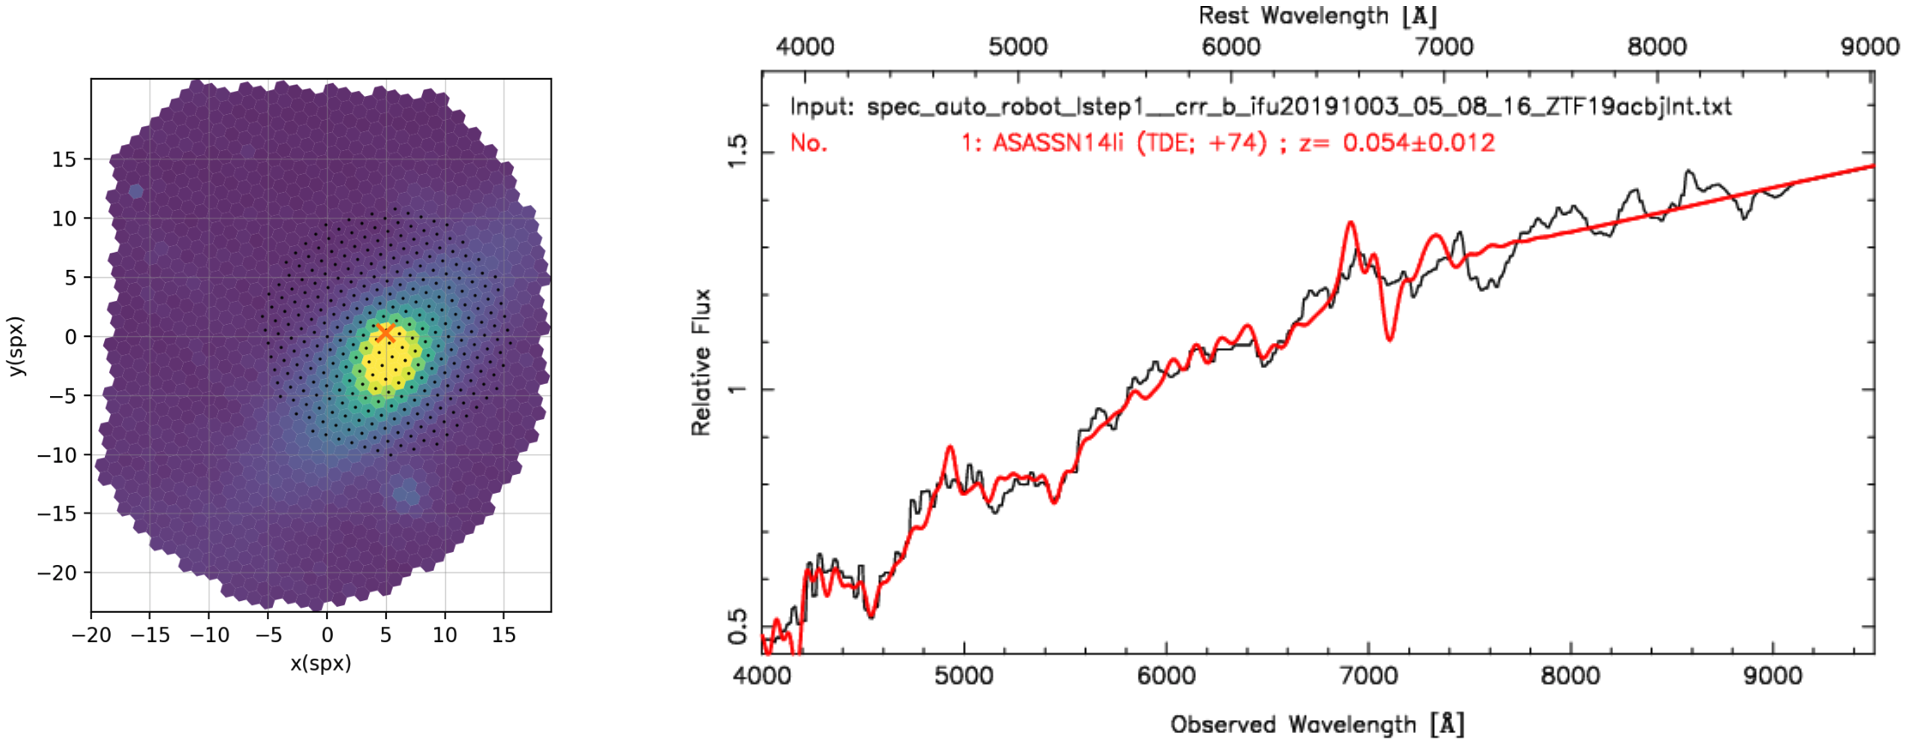
\includegraphics[width=0.95\textwidth]{../figures/03_sedm/stronghost.png}
  \caption[Exemple de situation extrême de contamination de supernova
  par la galaxie hôte]{Exemple de situation extrême de contamination de
    supernova par la galaxie hôte: ZTF19acbjlnt. \textit{À gauche} est représenté
    une image 2D du cube intégrée entre $[5000-8000]$\AA. La croix
    orange indique la position estimée de la supernova à partir des
    images de guidage de la RC. Les marqueurs noirs indiquent les
    spaxels considérés pour l'extraction de source ponctuelle. \textit{À droite} le spectre extrait en
    noir et la tentative de classification par \pkg{SNID}. On voit ici
    clairement que c'est à la fois le coeur de la galaxie et la
    supernova qui ont été extraits. L'extraction avec \pkg{contsep} ne
    change rien au résultat.}
  \label{fig:stronghost}
\end{figure}

Un moyen de lever cette contamination serait d'être en mesure de
modéliser la galaxie elle-même, afin de complètement isoler la source
ponctuelle dans le cube de données et ainsi procéder à une extraction
propre. 

%\bibliographystyle{../main/aa_url}
%\bibliography{99_references}
\end{document}

%%% Local Variables:
%%% mode: latex
%%% TeX-master: t
%%% End:
